\documentclass[10pt]{beamer}
\usetheme{metropolis}
\usepackage{booktabs}
\usepackage{tabularx}
\usepackage{calc}
\usepackage{tikz}
\usepackage{fontawesome5}

% Setup for faculty images
\newlength{\imageheight}
\setlength{\imageheight}{3.5cm}

% Define CSUF brand colors
\definecolor{titanblue}{HTML}{00244E}
\definecolor{mediumblue}{HTML}{0F3F8C}
\definecolor{skyblue}{HTML}{EBFBFF}
\definecolor{titanorange}{HTML}{FF7900}
\definecolor{titangray}{HTML}{F5F5F5}
\definecolor{titantext}{HTML}{222222}

% Additional colors for variety
\definecolor{accentcolor}{HTML}{E74C3C}
\definecolor{successcolor}{HTML}{27AE60}
\definecolor{dangercolor}{HTML}{DC3545}

% Customize metropolis theme colors
\setbeamercolor{normal text}{fg=titantext, bg=white}
\setbeamercolor{alerted text}{fg=titanorange}
\setbeamercolor{example text}{fg=mediumblue}

% Title page colors
\setbeamercolor{title}{fg=titanblue, bg=white}
\setbeamercolor{subtitle}{fg=mediumblue, bg=white}
\setbeamercolor{institute}{fg=titanorange, bg=white}
\setbeamercolor{date}{fg=titanblue, bg=white}

% Frame title colors
\setbeamercolor{frametitle}{fg=white, bg=titanblue}
\setbeamercolor{framesubtitle}{fg=mediumblue, bg=white}

% Block environment colors
\setbeamercolor{block title}{fg=white, bg=titanblue}
\setbeamercolor{block body}{fg=titantext, bg=skyblue!10}

% Alert block colors
\setbeamercolor{block title alerted}{fg=white, bg=dangercolor}
\setbeamercolor{block body alerted}{fg=titantext, bg=dangercolor!10}

% Item colors
\setbeamercolor{itemize item}{fg=titanorange}
\setbeamercolor{itemize subitem}{fg=mediumblue}
\setbeamercolor{itemize subsubitem}{fg=titanblue}

% Footer and header colors
\setbeamercolor{footer}{fg=titantext}
\setbeamercolor{header}{fg=titanblue}

% Customize fonts
\setbeamerfont{title}{size=\Large, series=\bfseries}
\setbeamerfont{frametitle}{size=\large, series=\bfseries}

% Simple title page template
\defbeamertemplate*{title page}{customized}[1][]
{
\vspace{1cm}
 {\usebeamerfont{title}\usebeamercolor[fg]{title}\inserttitle\par}
\vspace{0.5cm}
 {\usebeamerfont{subtitle}\usebeamercolor[fg]{subtitle}\insertsubtitle\par}
\vspace{0.5cm}
 {\usebeamerfont{date}\usebeamercolor[fg]{date}\insertdate\par}
\vfill
 {\insertinstitute\par}
}

% Add progress bar
\makeatletter
\setbeamertemplate{headline}{%
\begin{beamercolorbox}[wd=\paperwidth,ht=0.4cm,dp=0cm]{titanblue}%
\begin{tikzpicture}
\fill[titanorange] (0,0) rectangle (\the\paperwidth*\insertframenumber/\inserttotalframenumber,0.4cm);
\end{tikzpicture}%
\end{beamercolorbox}%
}
\makeatother

\begin{document}

\title{Policy Process Models}
\subtitle{Understanding How Policies Are Made\\POSC 315: Introduction to Public Policy\\Lecture 2 (Part 1 of 2)}
\date{Summer 2025}
\institute{California State University, Fullerton}

\maketitle

% Overview
\begin{frame}
\frametitle{Overview}

\begin{block}{Today's Focus:}
\begin{enumerate}
\item The Stages Model
\begin{itemize}
\item Structure and process
\item Strengths and limitations
\end{itemize}
\item Systems Thinking
\begin{itemize}
\item Systems model approach
\item Inputs, throughputs, and outputs
\item Strengths and limitations
\end{itemize}
\end{enumerate}
\end{block}

\pause
\vspace{0.5cm}
\centering
These models help us understand the complex process of policy development

\end{frame}

% The Stages Model - Overview
\begin{frame}
\frametitle{The Stages Model}

\vspace{0.5cm}
\begin{center}
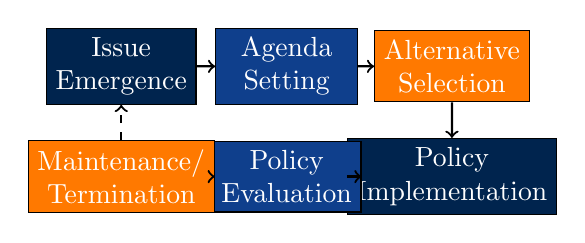
\begin{tikzpicture}[scale=0.7, every node/.style={align=center}]
% Draw the stages as connected boxes
\node[draw, rectangle, fill=titanblue, text=white, minimum width=1.8cm, minimum height=0.8cm] (issue) at (0,3) {Issue\\Emergence};
\node[draw, rectangle, fill=mediumblue, text=white, minimum width=1.8cm, minimum height=0.8cm] (agenda) at (3,3) {Agenda\\Setting};
\node[draw, rectangle, fill=titanorange, text=white, minimum width=1.8cm, minimum height=0.8cm] (selection) at (6,3) {Alternative\\Selection};
\node[draw, rectangle, fill=titanblue, text=white, minimum width=1.8cm, minimum height=0.8cm] (implement) at (6,1) {Policy\\Implementation};
\node[draw, rectangle, fill=mediumblue, text=white, minimum width=1.8cm, minimum height=0.8cm] (evaluate) at (3,1) {Policy\\Evaluation};
\node[draw, rectangle, fill=titanorange, text=white, minimum width=1.8cm, minimum height=0.8cm] (maintain) at (0,1) {Maintenance/\\Termination};

% Draw arrows
\draw[->, thick] (issue) -- (agenda);
\draw[->, thick] (agenda) -- (selection);
\draw[->, thick] (selection) -- (implement);
\draw[->, thick] (implement) -- (evaluate);
\draw[->, thick] (evaluate) -- (maintain);
\draw[->, thick, dashed] (maintain) -- (issue);
\end{tikzpicture}
\end{center}

\end{frame}

% The Stages Model - Details
\begin{frame}
\frametitle{The Stages Model}

\begin{columns}
\begin{column}{0.48\textwidth}
\begin{block}{First Stages}
\pause
\begin{itemize}
\item \textbf{Issue Emergence}: A problem is identified and brought to the attention of government
\item \textbf{Agenda Setting}: The problem is placed on the government agenda
\item \textbf{Alternative Selection}: Various policy options are considered
\end{itemize}
\end{block}
\end{column}

\begin{column}{0.48\textwidth}
\begin{block}{Later Stages}
\pause
\begin{itemize}
\item \textbf{Policy Implementation}: The policy is put into action
\item \textbf{Policy Evaluation}: Effectiveness is assessed
\item \textbf{Maintenance, Succession, or Termination}: Policy is continued, modified, or ended
\end{itemize}
\end{block}
\end{column}
\end{columns}

\pause
\vspace{0.5cm}
\centering
The process is cyclical, as new issues often emerge from existing policies

\end{frame}

% Stages Model Strengths
\begin{frame}
\frametitle{Stages Model Strengths}

\begin{columns}
\begin{column}{0.32\textwidth}
\begin{block}{\faCheck\ Intuitive}
\pause
Easy to understand and explain
\end{block}
\end{column}

\begin{column}{0.32\textwidth}
\begin{block}{\faCheck\ Descriptive}
\pause
Aligns with how people think about the policy process
\end{block}
\end{column}

\begin{column}{0.32\textwidth}
\begin{block}{\faCheck\ Flexible}
\pause
Adaptable to different policy areas and government levels
\end{block}
\end{column}
\end{columns}

\end{frame}

% Stages Model Weaknesses
\begin{frame}
\frametitle{Stages Model Weaknesses}

\begin{columns}
\begin{column}{0.32\textwidth}
\begin{alertblock}{\faTimes\ Linear}
\pause
Assumes a sequential process when reality is more complex
\end{alertblock}
\end{column}

\begin{column}{0.32\textwidth}
\begin{alertblock}{\faTimes\ Oversimplified}
\pause
Ignores much of the complexity in policymaking
\end{alertblock}
\end{column}

\begin{column}{0.32\textwidth}
\begin{alertblock}{\faTimes\ Separate}
\pause
Treats stages as distinct when they actually overlap
\end{alertblock}
\end{column}
\end{columns}

\end{frame}

% Reflection Point
\begin{frame}
\frametitle{Reflection Point}

\begin{block}{Think of a recent policy issue (e.g., COVID response, student debt):}
\begin{itemize}
\item Can you identify the different stages it went through?
\item Did it follow a linear path or move back and forth between stages?
\item Were some stages more visible or important than others?
\end{itemize}
\end{block}

\end{frame}

% Systems Thinking
\begin{frame}
\frametitle{Systems Thinking}

\begin{block}{}
A way of thinking about natural or social phenomena as a system with various inputs that are processed and intermingle to create a discernible set of outputs.
\end{block}

\pause
\begin{block}{}
A perspective that emphasizes the relationships among parts of a system and how they interact with each other and the system as a whole.
\end{block}

\pause
\vspace{0.5cm}
\centering
Rather than seeing policy as a linear sequence, systems thinking views it as a dynamic, interconnected process

\end{frame}

% The Systems Model
\begin{frame}
\frametitle{The Systems Model}

\begin{block}{}
\begin{itemize}
\item<1-> Public policy is viewed as the \textbf{response of the political system} to forces brought to bear on it from the outside environment.
\item<2-> A policy environment surrounds the political system
\begin{itemize}
\item Forces enter the political system from the environment either as demands or as support
\end{itemize}
\item<3-> The political system processes these inputs and produces policy outputs
\end{itemize}
\end{block}

\end{frame}

% Systems Model Diagram
\begin{frame}
\frametitle{The Systems Model}

\vspace{0.5cm}
\begin{center}
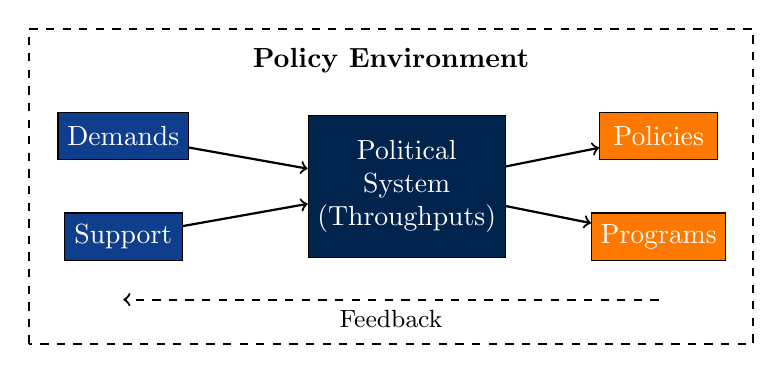
\begin{tikzpicture}[scale=0.8, every node/.style={align=center}]
% Environment box
\draw[thick, dashed] (-3.5,-2.5) rectangle (8,2.5);
\node at (2.25,2) {\textbf{Policy Environment}};

% Inputs
\node[draw, rectangle, fill=mediumblue, text=white, minimum width=1.5cm, minimum height=0.6cm] (demands) at (-2,0.8) {Demands};
\node[draw, rectangle, fill=mediumblue, text=white, minimum width=1.5cm, minimum height=0.6cm] (support) at (-2,-0.8) {Support};

% Political System (black box)
\node[draw, rectangle, fill=titanblue, text=white, minimum width=2.5cm, minimum height=1.8cm] (system) at (2.5,0) {Political\\System\\(Throughputs)};

% Outputs
\node[draw, rectangle, fill=titanorange, text=white, minimum width=1.5cm, minimum height=0.6cm] (policies) at (6.5,0.8) {Policies};
\node[draw, rectangle, fill=titanorange, text=white, minimum width=1.5cm, minimum height=0.6cm] (programs) at (6.5,-0.8) {Programs};

% Arrows
\draw[->, thick] (demands) -- (system);
\draw[->, thick] (support) -- (system);
\draw[->, thick] (system) -- (policies);
\draw[->, thick] (system) -- (programs);

% Feedback arrow
\draw[->, thick, dashed] (6.5,-1.8) -- (-2,-1.8);
\node at (2.25,-2.1) {\small Feedback};
\end{tikzpicture}
\end{center}

\vspace{0.3cm}
\centering
\small Note: This diagram illustrates the continuous feedback loops in the policy system

\end{frame}

% Systems Model Components
\begin{frame}
\frametitle{The Systems Model Components}

\begin{columns}
\begin{column}{0.48\textwidth}
\begin{block}{Environment \& Inputs}
\pause
\begin{itemize}
\item \textbf{Policy Environment}: Political, economic, social context
\item \textbf{Inputs}: Demands and support from public, interest groups, officials
\end{itemize}
\end{block}
\end{column}

\begin{column}{0.48\textwidth}
\begin{block}{Processing \& Results}
\pause
\begin{itemize}
\item \textbf{Throughputs}: The ``black box'' where processing occurs
\item \textbf{Outputs}: Laws, regulations, decisions created
\item \textbf{Outcomes}: Actual effects on society
\end{itemize}
\end{block}
\end{column}
\end{columns}

\pause
\vspace{0.3cm}
\begin{block}{Feedback}
Response to policy outputs that loops back into the system, potentially creating new demands or support
\end{block}

\end{frame}

% Systems Model Strengths
\begin{frame}
\frametitle{Systems Model Strengths}

\begin{columns}
\begin{column}{0.32\textwidth}
\begin{block}{1. Holistic}
\pause
Considers the entire environment and system interactions
\end{block}
\end{column}

\begin{column}{0.32\textwidth}
\begin{block}{2. Dynamic}
\pause
Acknowledges continuous interaction and feedback
\end{block}
\end{column}

\begin{column}{0.32\textwidth}
\begin{block}{3. Flexible}
\pause
Adaptable to various policy contexts and levels
\end{block}
\end{column}
\end{columns}

\end{frame}

% Systems Model Weaknesses
\begin{frame}
\frametitle{Systems Model Weaknesses}

\begin{columns}
\begin{column}{0.48\textwidth}
\begin{alertblock}{1. Complex}
\pause
Difficult to apply in practice due to its comprehensive nature
\end{alertblock}
\end{column}

\begin{column}{0.48\textwidth}
\begin{alertblock}{2. Abstract}
\pause
Does not provide clear explanation of specific processes
\end{alertblock}
\end{column}
\end{columns}

\pause
\vspace{0.5cm}
\centering
The ``black box'' of processing remains somewhat unclear

\end{frame}

% Comparing the Models
\begin{frame}
\frametitle{Comparing the Models}

\begin{table}
\centering
\begin{tabular}{|l|l|l|}
\hline
\textbf{Feature} & \textbf{Stages Model} & \textbf{Systems Model} \\
\hline
\pause
Structure & Linear, sequential & Dynamic, interconnected \\
\hline
\pause
Focus & Process steps & Environmental interactions \\
\hline
\pause
Complexity & Simple, intuitive & Complex, holistic \\
\hline
\pause
Best Use & Instructional, basic analysis & Complex policy analysis \\
\hline
\end{tabular}
\end{table}

\end{frame}

% Key Takeaways
\begin{frame}
\frametitle{Key Takeaways}

\begin{block}{}
\begin{itemize}
\item \textbf{Stages Model}: Provides a useful framework but oversimplifies reality
\item \textbf{Systems Model}: Emphasizes relationships, feedback loops, and environmental context
\item \textbf{Complementary Views}: Both models provide valuable insights while having distinct limitations
\item \textbf{Practical Application}: Understanding these models helps analyze real-world policy development
\end{itemize}
\end{block}

\vspace{1cm}

\begin{quotation}
``Models are to be used, not believed.''

\vspace{0.3cm}
\hfill --- Henri Theil
\end{quotation}

\end{frame}

% Coming Up Next
\begin{frame}
\frametitle{Coming Up Next}
\framesubtitle{In Part 2, we'll examine the specific environments that shape policy decisions:}

\begin{columns}
\begin{column}{0.48\textwidth}
\begin{block}{We'll Cover:}
\begin{itemize}
\item Structural Environment
\item Social Environment
\item Economic Environment
\item Political Environment
\item International Environment
\end{itemize}
\end{block}
\end{column}

\begin{column}{0.48\textwidth}
\begin{block}{Questions to Consider:}
\begin{itemize}
\item How do environments constrain policy choices?
\item Which environmental factors are most influential?
\item How do these environments interact?
\end{itemize}
\end{block}
\end{column}
\end{columns}

\end{frame}

\end{document}